\subsubsection{Construction of the Experiment}

\begin{figure}
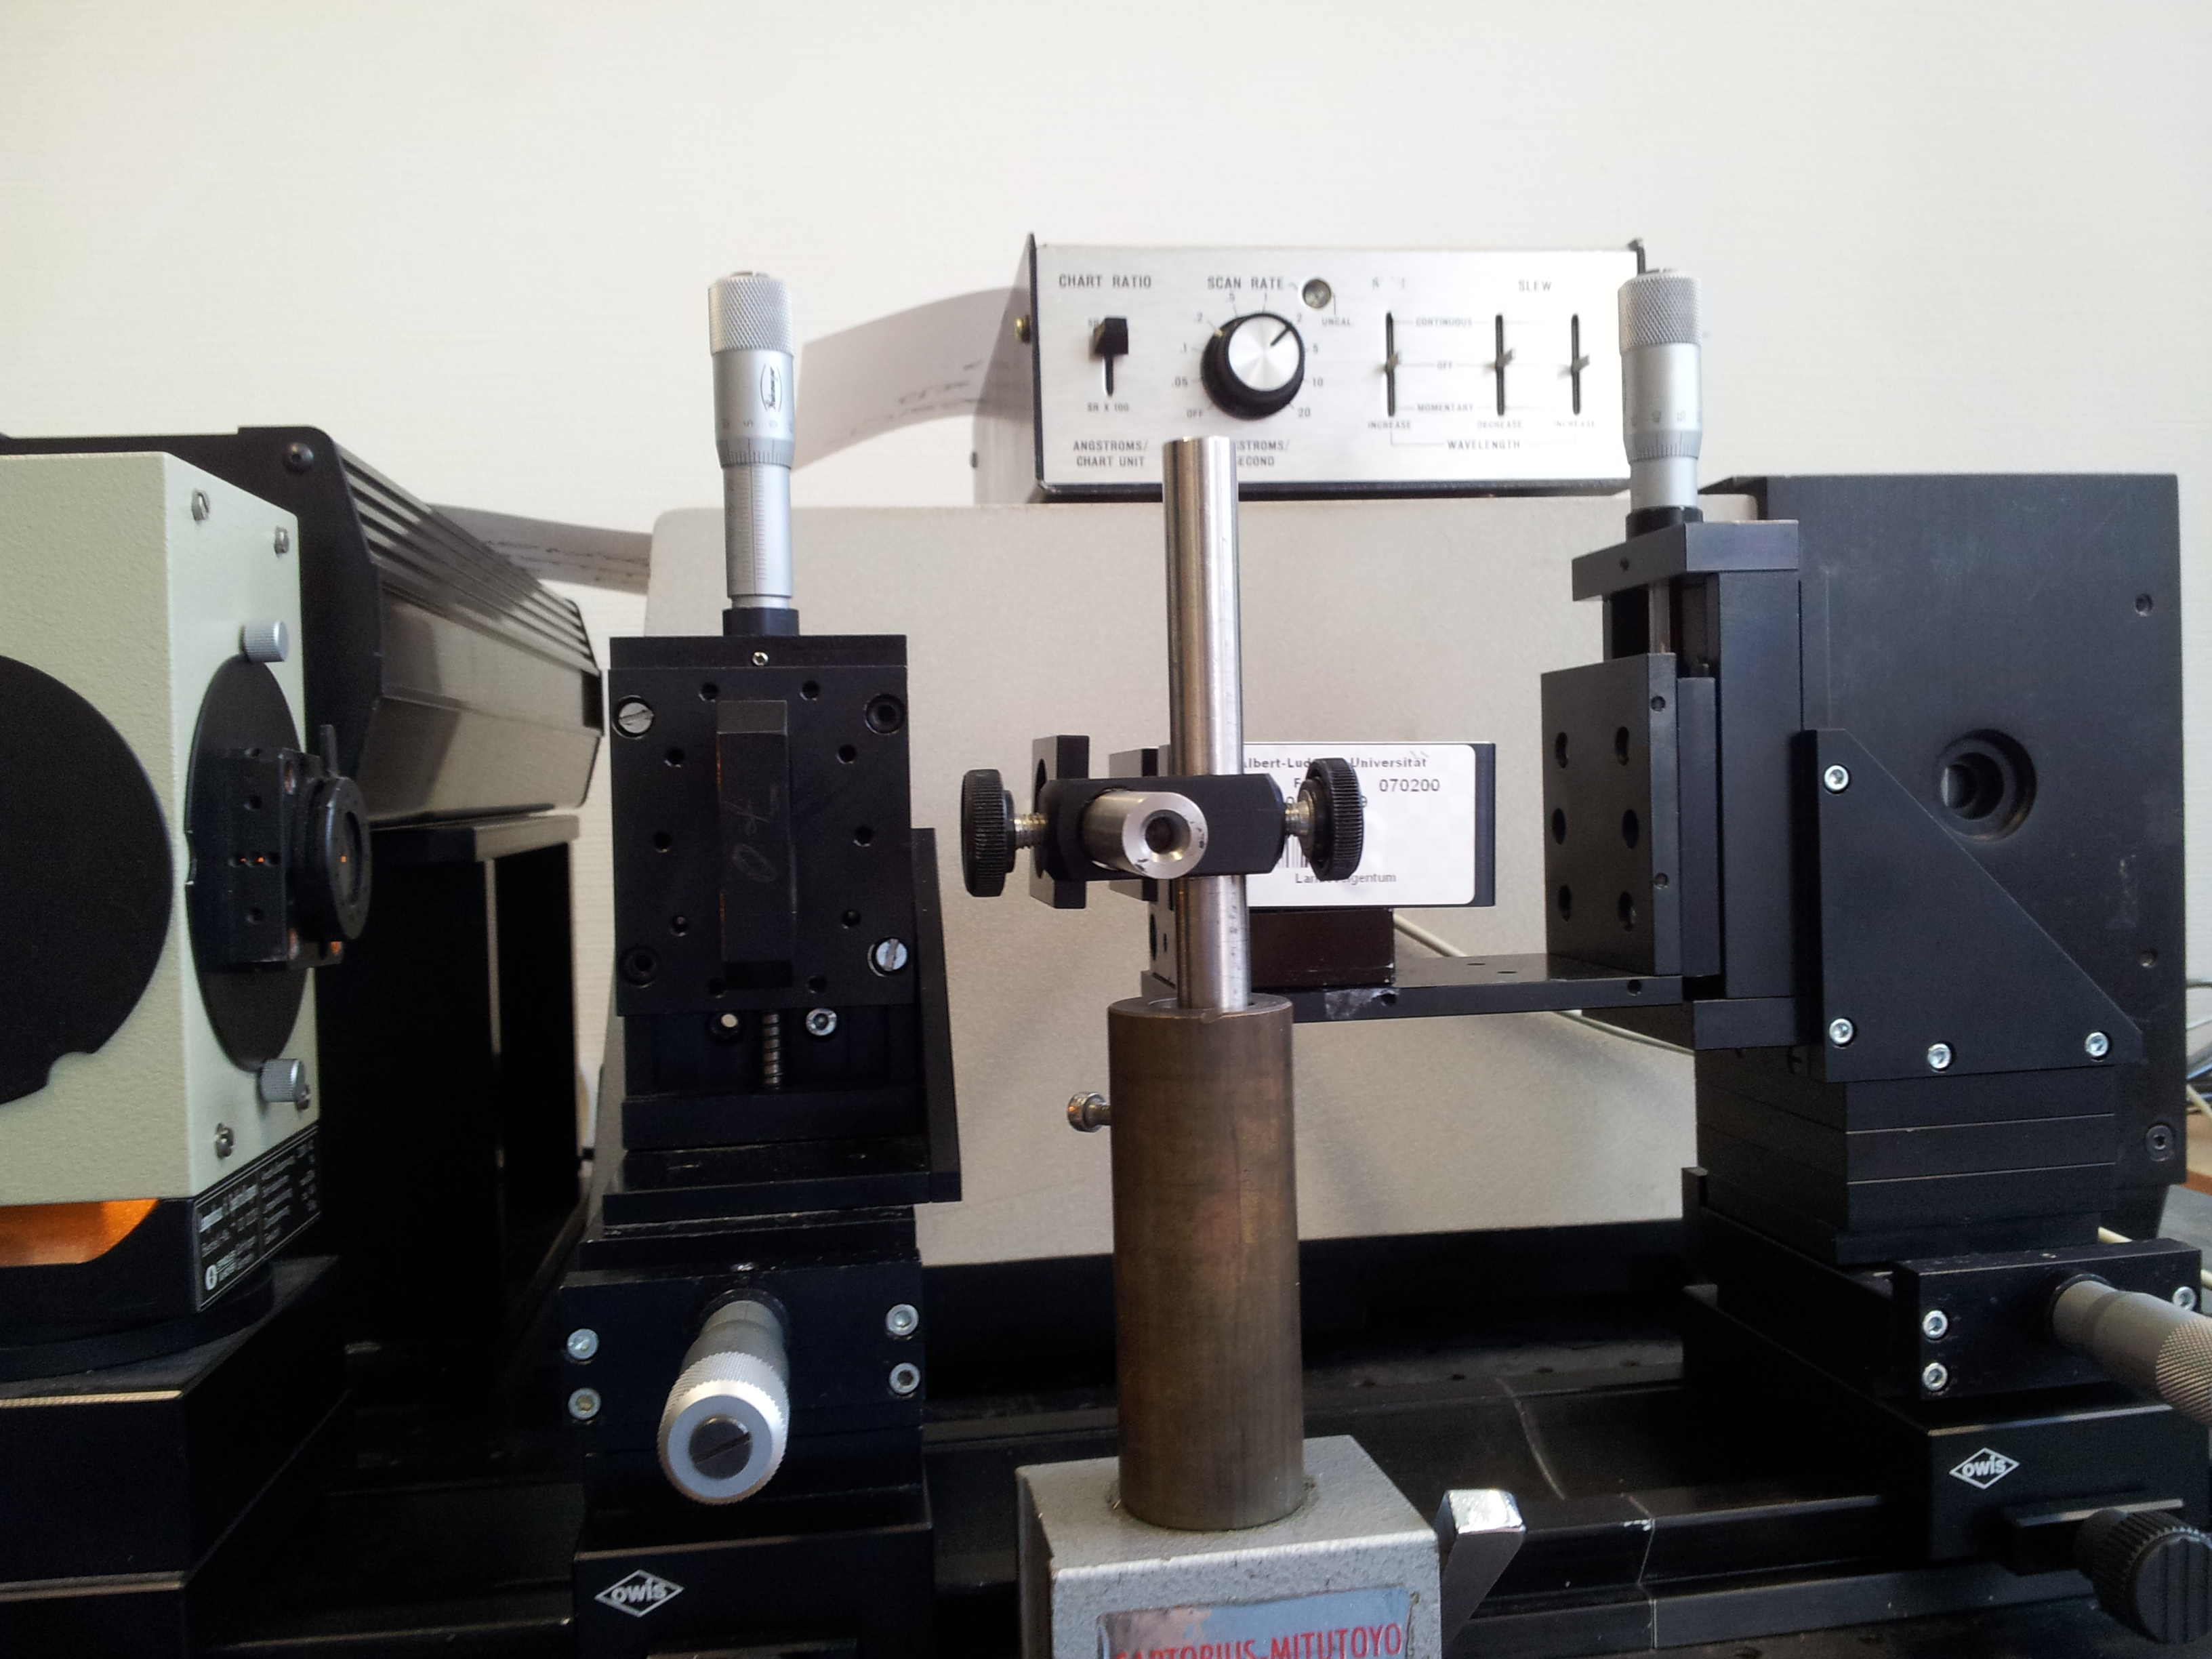
\includegraphics[width=10cm]{pics/const1}
\caption{Construction of the Experiment (a)}
\label{fig:const1}
\end{figure}
\begin{figure}
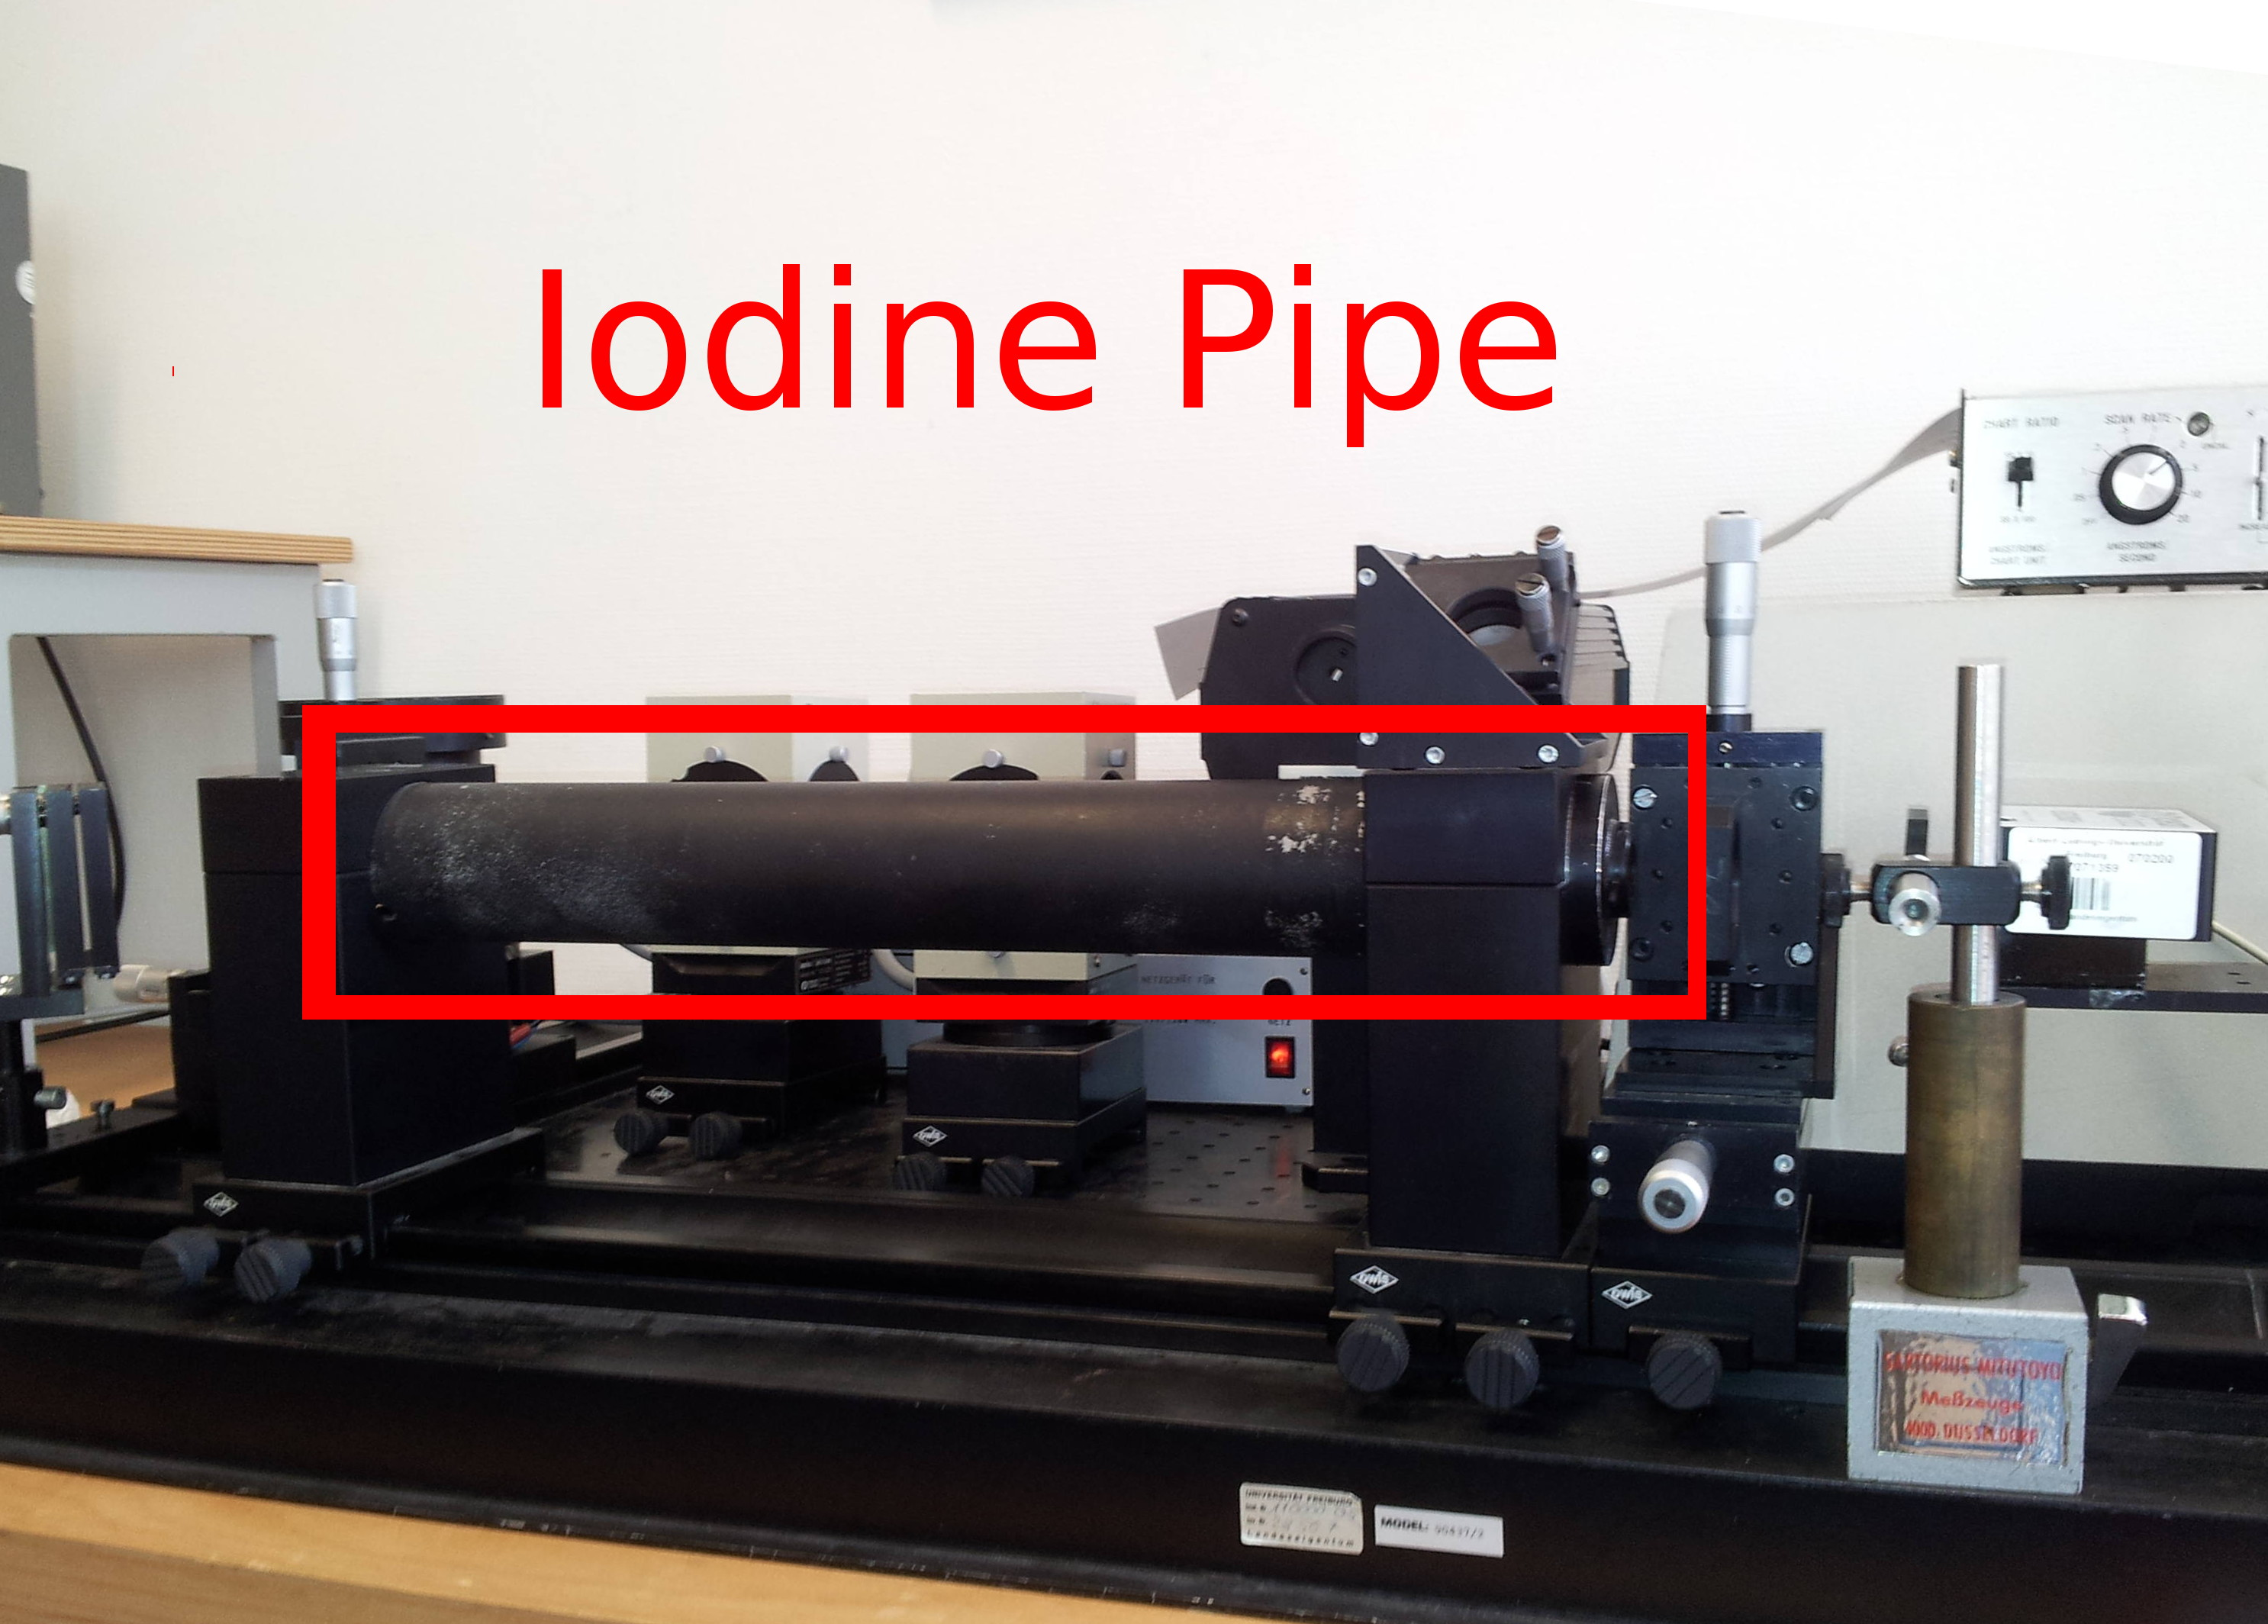
\includegraphics[width=10cm]{pics/const2}
\caption{Construction of the Experiment (a)}
\label{fig:const2}
\end{figure}
\begin{figure}
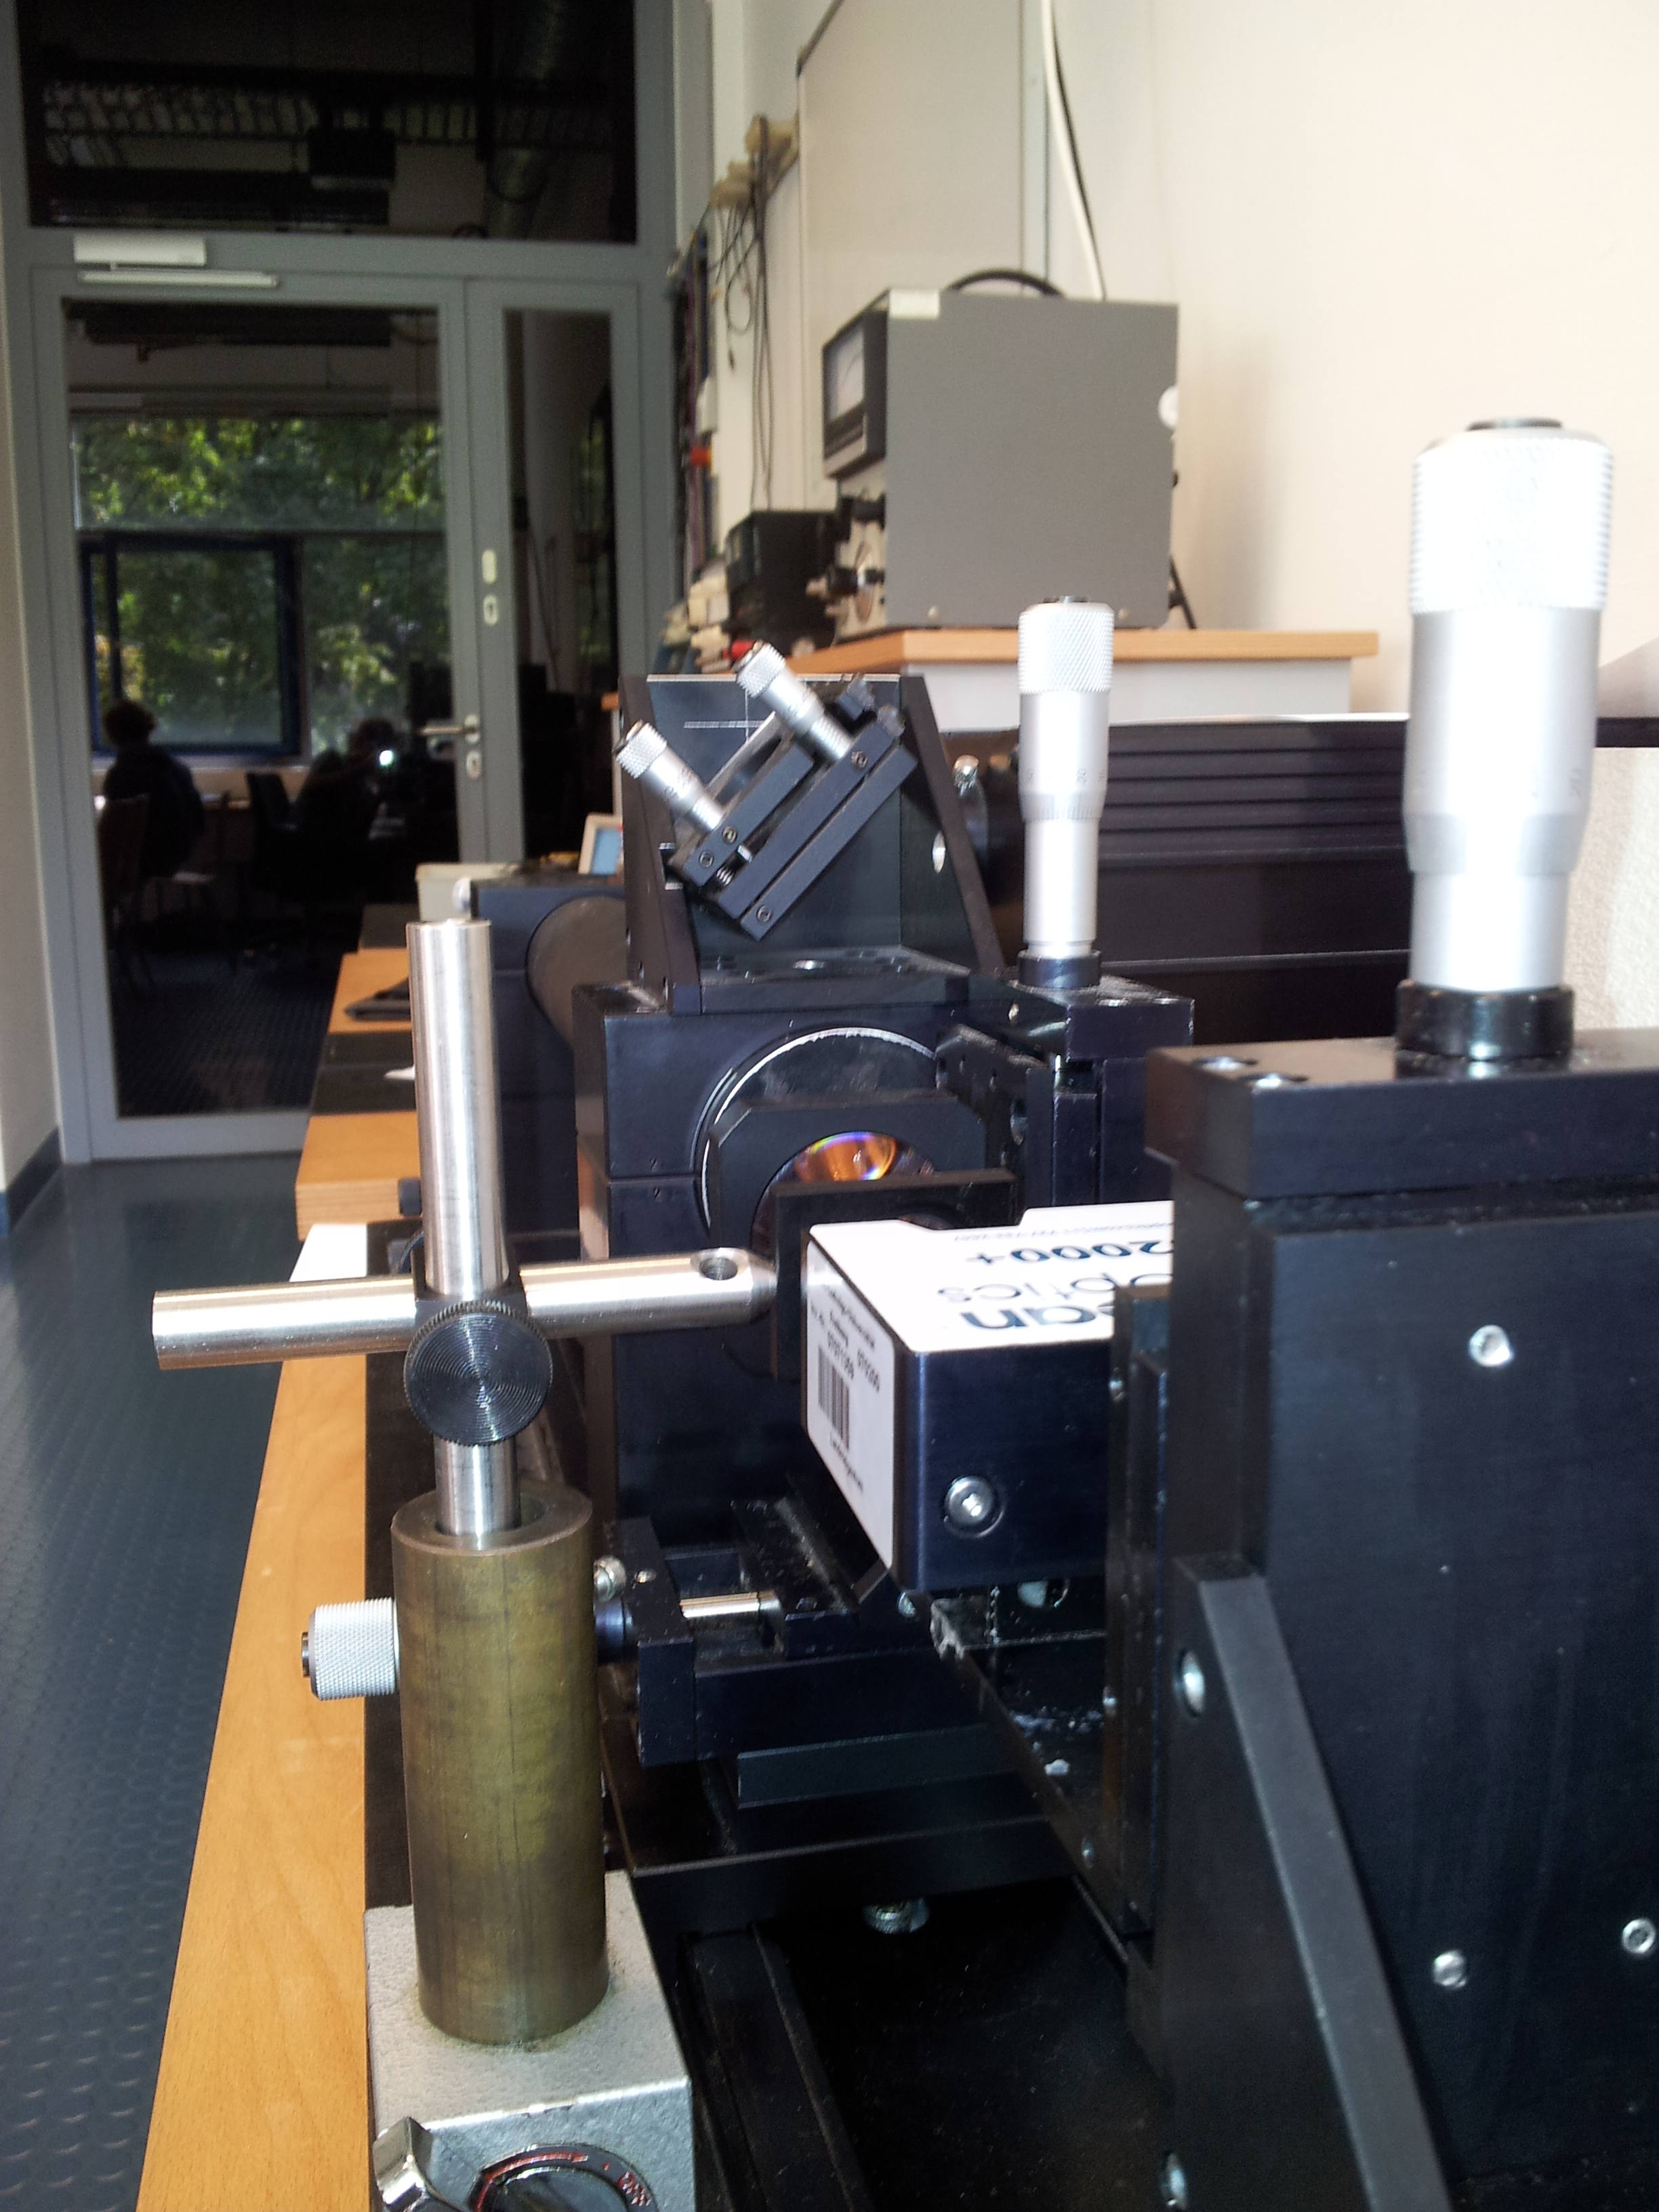
\includegraphics[width=10cm]{pics/const3}
\caption{Construction of the Experiment (a)}
\label{fig:const3}
\end{figure}
\begin{figure}
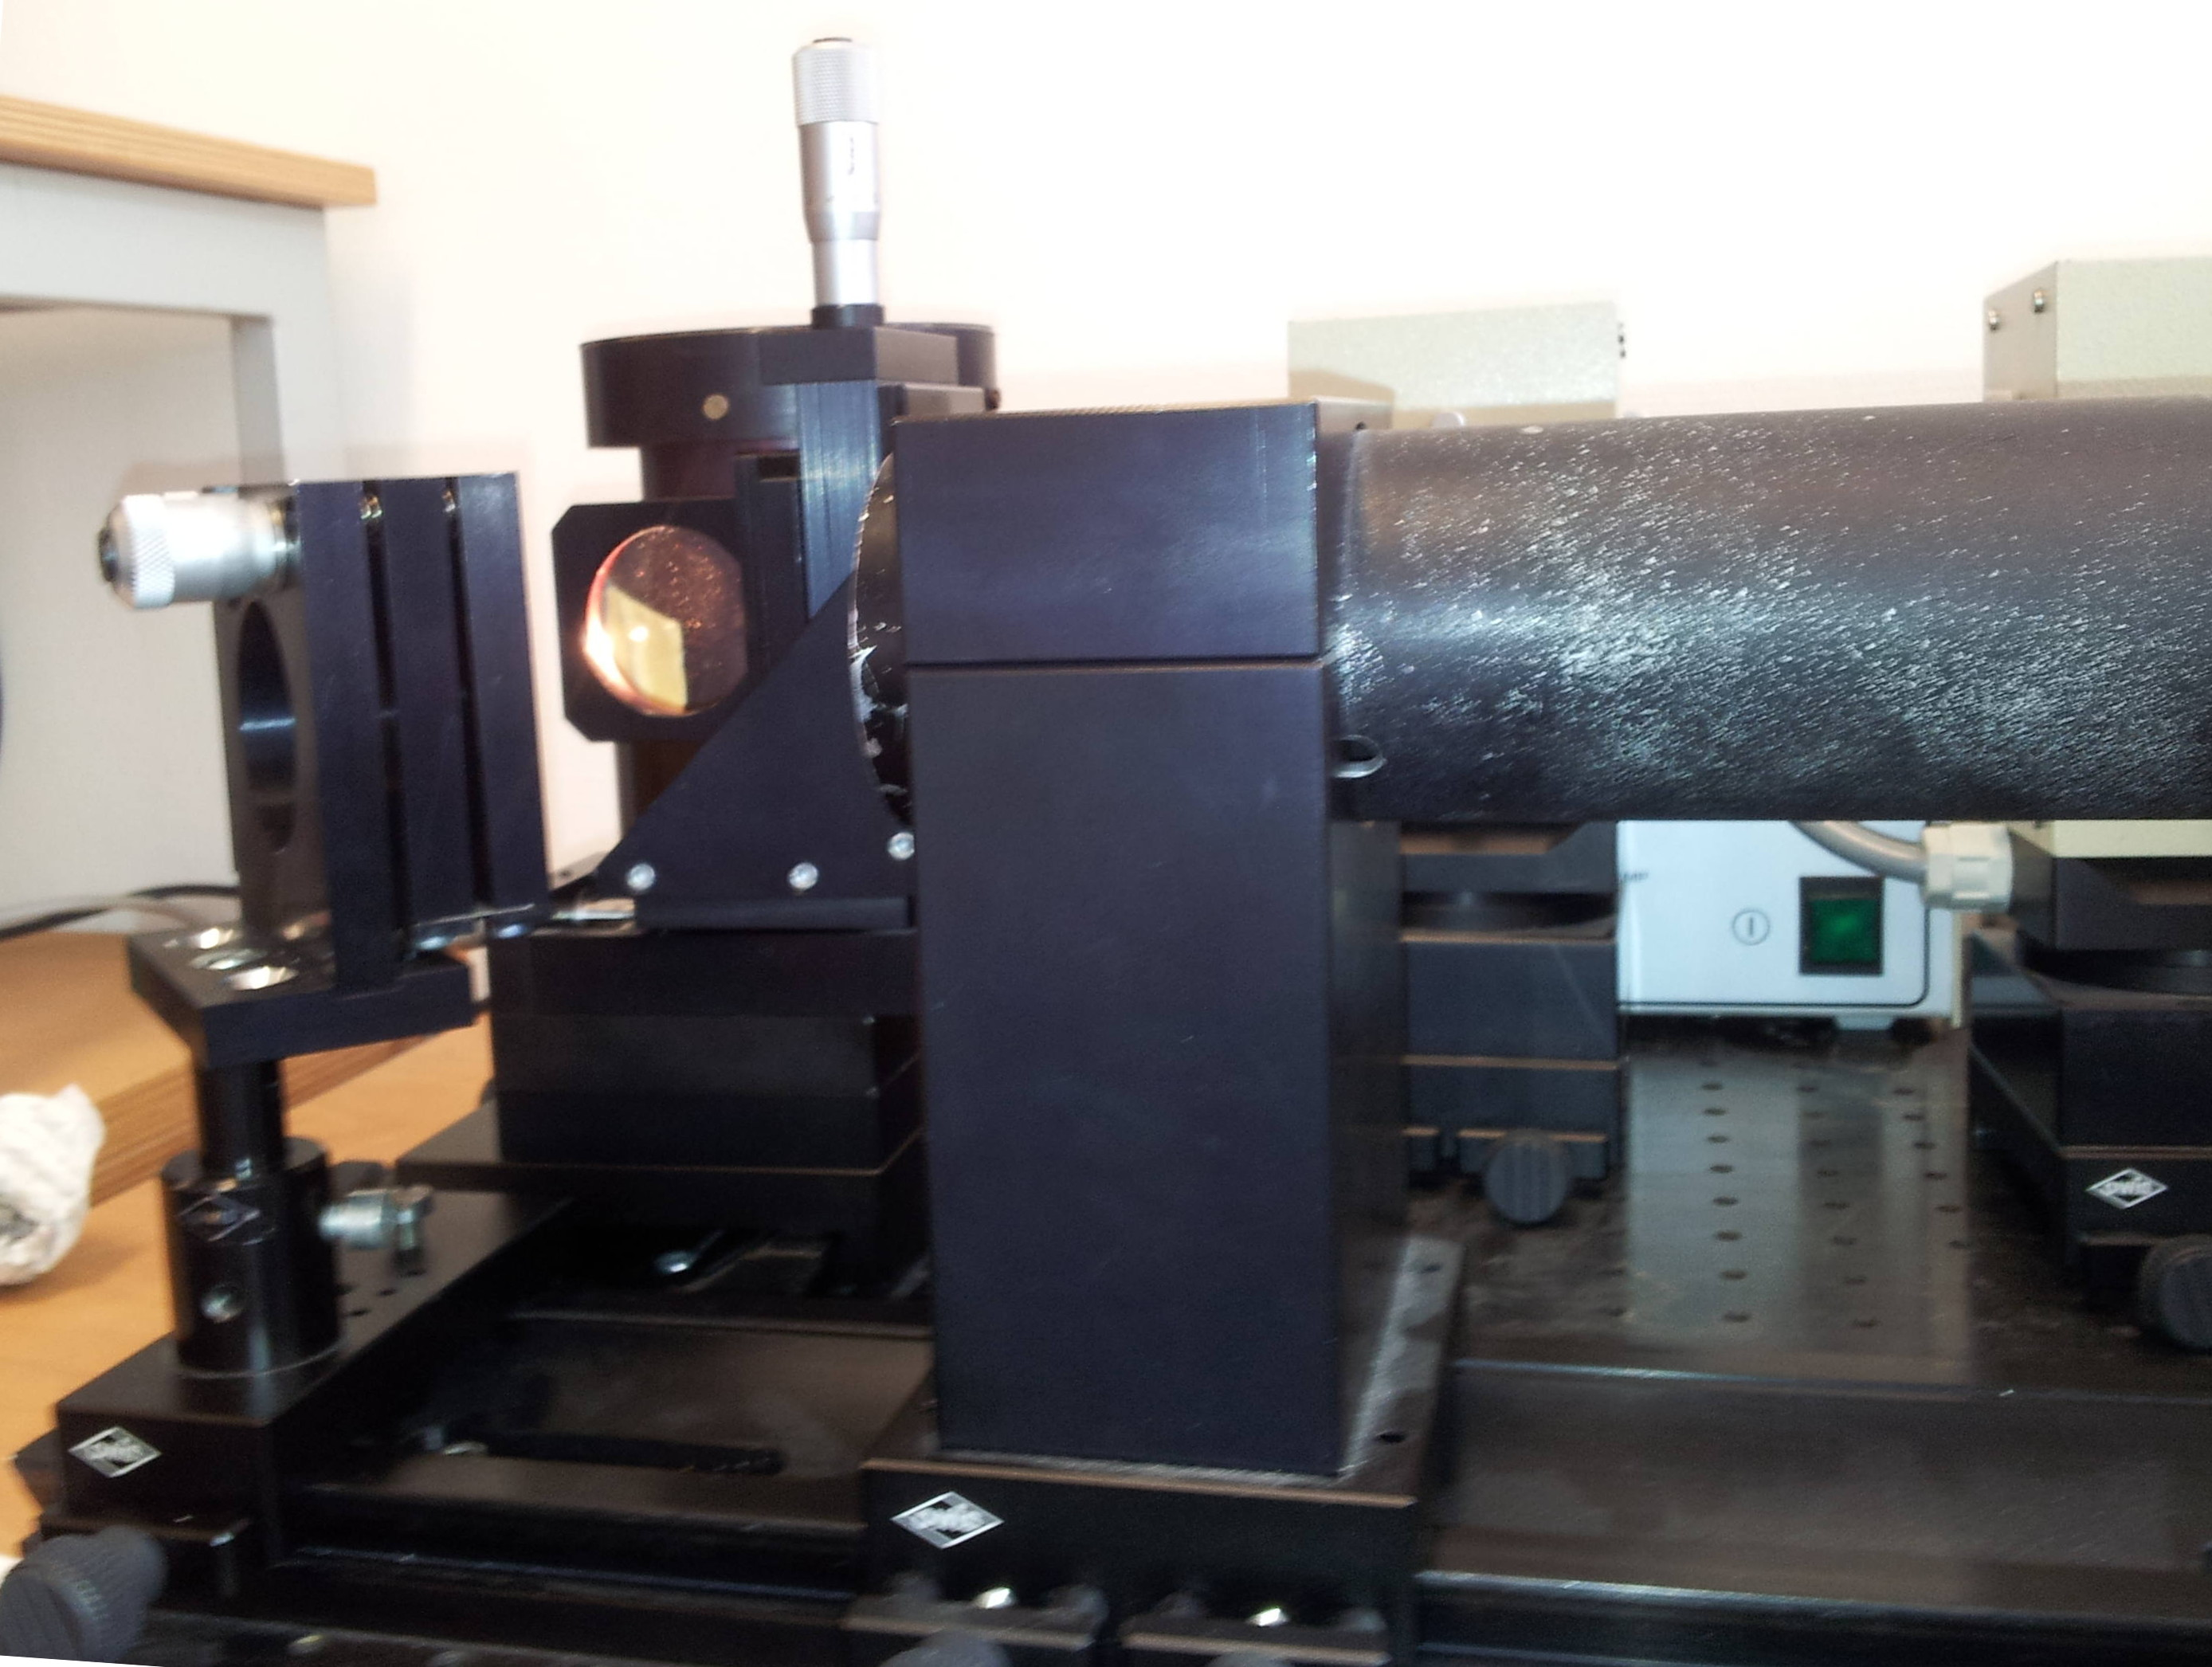
\includegraphics[width=10cm]{pics/const4}
\caption{Construction of the Experiment (a)}
\label{fig:const4}
\end{figure}
\begin{figure}
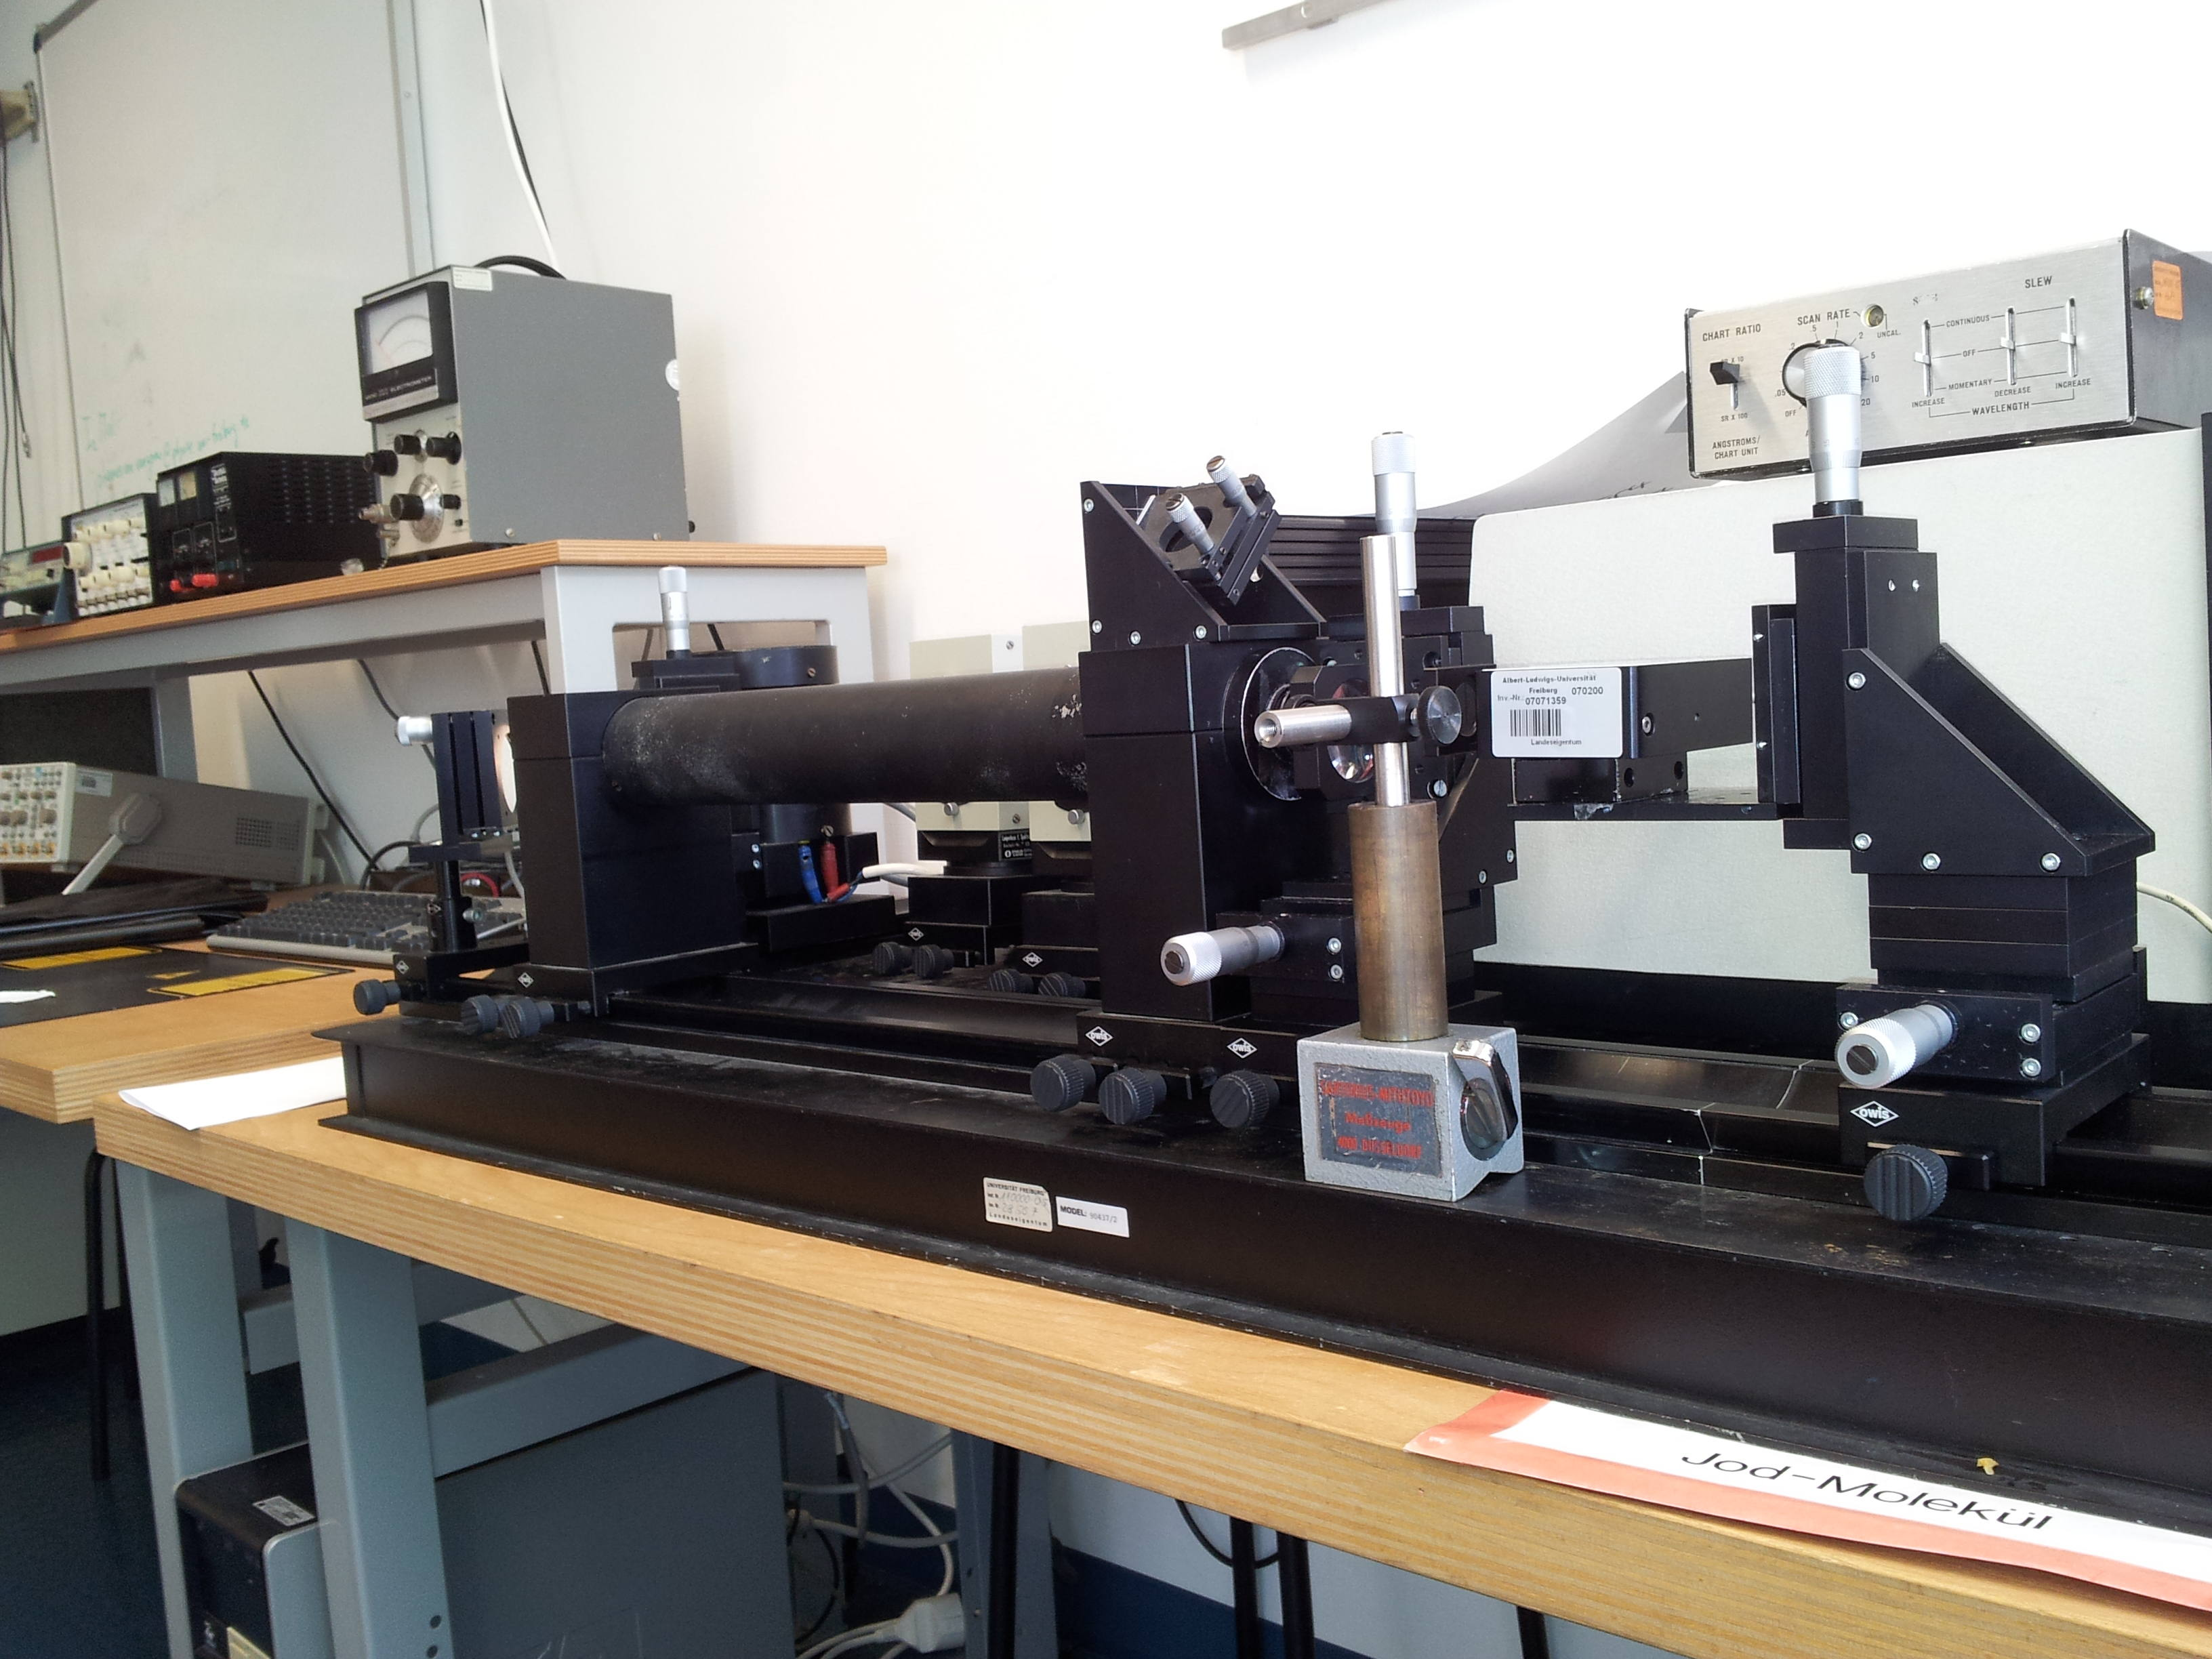
\includegraphics[width=10cm]{pics/const_overview}
\caption{Construction of the Experiment (a)}
\label{fig:const_overview}
\end{figure}

